Escribe una expresión para calcular el perímetro y el área de la figura \ref{fig:20230319044600}

\begin{figure}[H]
    \centering
    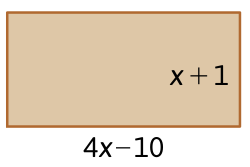
\includegraphics[width=0.25\textwidth]{../images/20230319044600}
    \caption{}
    \label{fig:20230319044600}
\end{figure}


\begin{solutionbox}{3.5cm}
    \begin{multicols}{2}
      Perímetro:
      \begin{align*}
        P & =2(4x-10)+2(x+1) \\
          & =8x-20+2x+2      \\
          & =10x-18
        \end{align*}

      Área:
      \begin{align*}
        A & =(4x-10)(x+1)     \\
          & =4x^2-10x+4x-10  \\
          & =4x^2-6x-10
      \end{align*}
    \end{multicols}
  \end{solutionbox}